\documentclass[a4paper,12pt,twocolumn,landscape]{article}

\usepackage{superpack2015}

\usepackage[heightrounded]{geometry}	% heightrounded permet d'afficher les footers correctement
\geometry{hmargin=0.5cm,vmargin=1.5cm}

\setlength{\columnseprule}{0.5pt}		% Ligne séparatrice milieu document
\setlength{\columnsep}{50pt}			% Espace de chaque côté de la ligne
\setlength{\headsep}{15pt}
\addtolength{\textheight}{20pt}
%\setlength{\textwidth}{770pt}
%\setlength{\hoffset}{20pt}

\classichf
	% Nom du style
	{premierepage}
	% Hauteur sous header
	% 14.5pt si une ligne (1 \baselineskip)
	% 29.0pt si deux lignes (2 \baselineskip)
	{14.5pt}
	% Head
	{}
	{\textbf{Exercices : Repérage das le plan}}
	{}
	% Foot
	{a}
	{a}
	{a}

\usepackage{showframe}
%\usepackage{layout}

\begin{document}
\pagestyle{premierepage}	%\thispagestyle{premierepage} pour isoler des styles de pages

%\exercice Placez 2 points $A$ et $B$ et tracez le vecteur~\vectaffiche{AB}.
\begin{enumerate}
	\item Construisez un vecteur opposé à \vectaffiche{AB}.
	\item Construisez un vecteur de même direction et de même sens que \vectaffiche{AB} et qui n'est pas égal à \vectaffiche{AB}.
	\item Construisez un vecteur de même direction que \vectaffiche{AB} mais de sens contraire et qui n'est pas égal à \vectaffiche{BA}.
\end{enumerate}
%\exercice À partir de la figure ci-dessous,
\begin{enumerate}
	\item donnez les images des points $C$, $D$ et $E$ par la translation de~vecteur~\vectaffiche{AB},
	\item citez 3 vecteurs égaux au vecteur \vectaffiche{AB},
	\item citez 3 parallélogrammes ayant $A$ et $B$ parmi leurs sommets et définis par les égalités vectorielles de la question précédente.
\end{enumerate}
\begin{center}
	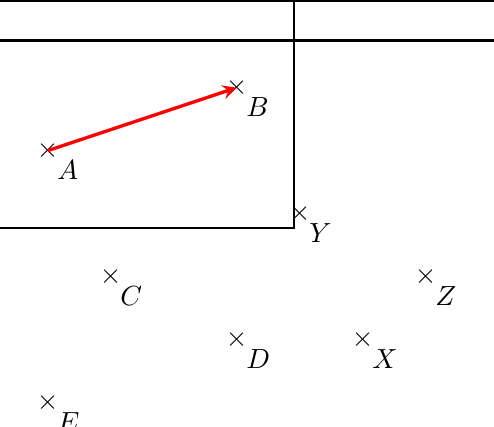
\begin{tikzpicture}[scale=0.8,every node/.style={scale=1}]
	\tikzstyle{vect}=[->,>=stealth,very thick]
	\tikzstyle{vectred}=[vect,red]
	\tikzstyle{etiquette}=[fill=white,
							midway,
							sloped,
							above]
								
\grille{0}{0}{9}{7}{thick};

\coordinate (A) at (2,5);
\coordinate (B) at (5,6);
\coordinate (C) at (3,3);
\coordinate (D) at (5,2);
\coordinate (E) at (2,1);
\coordinate (X) at (7,2);
\coordinate (Y) at (6,4);
\coordinate (Z) at (8,3);
\foreach \point in {A, ..., E, X, Y, Z}
	\draw (\point) node{$\times$} node[below right]{$\point$};
	
\draw[vectred] (A) -- (B);

\end{tikzpicture}
\end{center}
%\exercice Construisez un carré $ABCD$ de côté 5~carreaux et de centre~$O$. Construisez ensuite l'image de ce carré~:
\begin{enumerate}
	\item (en noir) par la translation de vecteur \vectaffiche{AB}
	\item (en bleu) par la translation de vecteur \vectaffiche{DB}
	\item (en vert) par la translation de vecteur \vectaffiche{OB}
\end{enumerate}
%\exercice Placez 3 points $A$, $B$ et $C$, tracez le triangle $ABC$ puis construisez l'image de ce triangle par la translation de vecteur \vectaffiche{CA}.
%\exercice À partir de la figure ci-dessous, citez un vecteur~:
\begin{enumerate}
	\item opposé à \vectaffiche{CD},
	\item de même direction et de même sens que \vectaffiche{AC},
	\item de même direction que \vectaffiche{BC} mais de sens contraire,
	\item égal au vecteur \vectaffiche{BA}.
\end{enumerate}

\begin{center}
	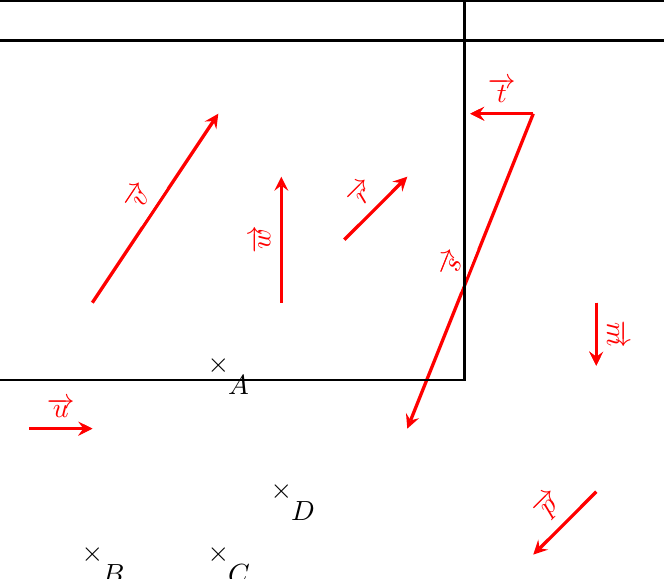
\begin{tikzpicture}[scale=0.8,every node/.style={scale=1}]
	\tikzstyle{vect}=[->,>=stealth,very thick]
	\tikzstyle{vectred}=[vect,red]
	\tikzstyle{etiquette}=[fill=white,
							midway,
							sloped,
							above]
								
\grille{0}{0}{10}{9}{thick};

\coordinate (A) at (3,4);
\coordinate (B) at (1,1);
\coordinate (C) at (3,1);
\coordinate (D) at (4,2);
\foreach \point in {A, ..., D}
	\draw (\point) node{$\times$} node[below right]{$\point$};
	

\draw[vectred] (9,5) -- ++ (0,-1) node[etiquette]{$\overrightarrow{m}$};
\draw[vectred] (9,5) -- ++ (0,-1); % on repasse la fleche car fleche trop courte

\draw[vectred] (9,2) -- ++ (-1,-1) node[etiquette]{$\overrightarrow{p}$};

\draw[vectred] (5,6) -- ++ (1,1) node[etiquette]{$\overrightarrow{r}$};

\draw[vectred] (8,8) -- ++ (-2,-5) node[etiquette]{$\overrightarrow{s}$};

\draw[vectred] (8,8) -- ++ (-1,0) node[etiquette]{$\overrightarrow{t}$};
\draw[vectred] (8,8) -- ++ (-1,0);

\draw[vectred] (0,3) -- ++ (1,0) node[etiquette]{$\overrightarrow{u}$};
\draw[vectred] (0,3) -- ++ (1,0);

\draw[vectred] (1,5) -- ++ (2,3) node[etiquette]{$\overrightarrow{v}$};

\draw[vectred] (4,5) -- ++ (0,2) node[etiquette]{$\overrightarrow{w}$};

\end{tikzpicture}
\end{center}
%\exercice (figure de l'exercice précédent)
\begin{enumerate}
	\item Placez les points $E$, $F$, $G$ et $H$, images respectives du point $A$ par les translations de vecteurs~:
	\begin{inparaenum}\\
		\hspace*{0pt}
		\item \vectaffiche{w}\hspace*{\stretch{1}}
		\item \vectaffiche{v}\hspace*{\stretch{1}}
		\item \vectaffiche{p}\hspace*{\stretch{1}}
		\item \vectaffiche{m}\hspace*{\stretch{1}}~
	\end{inparaenum}
	\item Placez les points $I$, $J$, $K$ et $L$, images respectives du point $B$ par les translations de vecteurs~:
	\begin{inparaenum}\\
		\hspace*{0pt}
		\item \vectaffiche{r}\hspace*{\stretch{1}}
		\item \vectaffiche{u}\hspace*{\stretch{1}}
		\item \vectaffiche{w}\hspace*{\stretch{1}}
		\item \vectaffiche{m}\hspace*{\stretch{1}}~
	\end{inparaenum}
	\item En utilisant les lettres de la figure~:
	\begin{enumerate}
		\item citez 2 vecteurs égaux à \vectaffiche{AB}
		\item citez 2 vecteurs opposés à \vectaffiche{AB}
	\end{enumerate}
\end{enumerate}

\exercice

\end{document}


%
%%\exercicebareme{4}
%\exercicebareme{6}
%\exercicebareme{10}
%\exerciceunpoint
%\exercicebonus
%\FIN
%\BONNESVACANCES
%\hrulefill